\chapter{Related Work}
\label{sec:related}
% Of course much work in this field and cannot possibly cover all of this so confined to closely related or well-known / state of the art
The demand for aid in the process of selecting an algorithm has already led to the development of a number of solutions that automate machine-learning (AutoML). In the following sections, the functionality of a few such tools that are related to this work are outlined briefly, organized by their scope of operation. Each tool's usage of meta knowledge is discussed shortly.

\section{Predicting Rankings}
%% Ranking
% Incorporating times
In contrast to ranking solely based on classifier performances, \citeauthor{DBLP:journals/ml/AbdulrahmanBRV18} investigated an approach to extend existing ranking methods by incorporating the time needed for the evaluation of the classifiers \cite{DBLP:journals/ml/AbdulrahmanBRV18}. They call this combined measure of accuracy and time A3R, and integrate it into two different ranking approaches. In both cases, the authors find that this leads to a better mean interval loss, which is a measure that expresses the mean loss experienced with respect to the time that has been allowed for the construction of the ranking, that is the time taken to evaluate top-ranked classifiers. 

% Rank aggregation A3R
One of those two approaches is called average-ranking. It utilizes meta knowledge to suggest a ranking of classifiers for a new data set, which in this case consists of recorded past performances of classifiers on a number of data sets, meaning this algorithm aggregates the performances of classifiers across all data sets once and then always recommends the same ranking. The new measure is integrated here by, instead of ordering only according to performance values, ordering classifiers according to the combined measure A3R.

% Active testing A3R
The second approach does not initially use meta knowledge and is called active testing. Active testing is a strategy that 'intelligently selects the most useful tests' \cite{DBLP:journals/ml/AbdulrahmanBRV18} to perform on a given data sets. Tests in this context mean the evaluation of a classifier that is considered for the ranking on the given data set. The authors improved this strategy by reducing the time needed to identify a good algorithm by, similarly to the rank aggregation variant, incorporating time in the estimations made by the strategy which previously only compared accuracy values.

\section{Algorithm and Hyperparameter Selection}
%% CASH
Taking it a step further than predicting rankings of classification algorithms with fixed hyperparameters is additionally also optimizing the classifier's hyperparameters, which has been defined as 'the combined algorithm selection and hyperparameter optimization problem (short: CASH)' \cite{thornton2013auto}. Two widely used approaches of this kind are Auto-WEKA and AUTO-SKLEARN. It has to be noted that thus these approaches also go further than the solution proposed in this thesis, which currently only takes into account one fixed hyperparameter configuration for each classification algorithm. 

% Auto-WEKA
Auto-WEKA is an AutoML tool that both selects a machine learning algorithm and optimizes its hyperparameters by using Bayesian optimization \cite{thornton2013auto}. It was first released in 2013 as an extension to the popular data mining software WEKA \cite{hall2009weka}, which also offers a user-friendly GUI in addition to a command-line interface and an API, to assist the large number of novice users of the software in selecting parametrized algorithms for their problems. The tool has since grown in popularity and is in version 2.0 as of March 2016 \cite{kotthoff2016auto}. In Auto-WEKA, the problem of selecting an algorithm and its hyperparameters is combined by treating the algorithm itself as a hyperparameter and searching the joint space of algorithms and hyperparameters for the best solution. An input data set is first preprocessed by means of feature selection. Then, Sequential Model-Based Optimization for General Algorithm Configuration (SMAC) is used to 'iterate[...] between fitting models and using them to make choices about which configurations to investigate' \cite{hutter2011sequential}. In the case of Auto-WEKA, this means that during the optimization process, a model is built, a configuration of hyperparameters that is promising regarding the current model and training data is tried out, and the result is fed back to the model. This cycle is then repeated until the allocated time has run out. Auto-WEKA exploits hard-coded meta-knowledge, that is considering past performances of algorithms, to make decisions by always trying algorithms like Random Forest, which perform well on a large number of data sets, first. \\

% SK-learn
AUTO-SKLEARN has been described as a sister-package to Auto-WEKA and is an AutoML tool which is based on scikit-learn, a machine learning library for Python \cite{feurer2015efficient}. It works very similar to AutoML but extends it by adding a meta-learning pre-processing step to warmstart the Bayesian optimization and automatically constructing ensembles during optimization. During the pre-processing phase, performance values for the classifiers available in AUTO-SKLEARN are recorded on a set of data sets. For each data set, the algorithm which shows the best empirical performance is noted. Then, certain meta-features are calculated for each data set. The first step of the tool when given a new problem is to calculate meta-features of the data set. Then, the Manhattan distance to the other data sets is determined according to the meta-features, and the algorithms that are associated with the k-nearest data sets are used as a starting point for further optimization. The authors observe that the additional meta-learning and ensemble construction result in a more efficient and robust application. Their results show that meta-learning can be used to improve the overall AutoML process.\\

\section{Constructing pipelines}
%% Whole pipelines
Before a classifier is evaluated on a data set, often a number of pre-processing steps are executed first. This includes, for example, selecting promising features and discarding others, and normalizing the data. The 'sequence of tasks that need to be performed to classify instances belonging to a given dataset into a set of predefined categories' \cite{DBLP:conf/eurogp/SaPOP17} can therefore be defined as a machine learning pipeline. Two tools which construct such complete pipelines for data sets are ML-Plan and the RECIPE framework.

% ML-Plan
ML-Plan is an AutoML tool that instead of concentrating on hyperparameter optimization, aims to optimize the whole machine-learning pipeline \cite{wever2017automatic}. This is achieved by viewing machine-learning as a task, building a hierarchical task network out of the resulting subtasks, and then searching for a solution in the induced tree structure. In the tree, the root node contains the complex task of building a machine learning pipeline, inner nodes represent incomplete pipelines consisting of complex and possibly also primitive tasks, and leaf nodes are complete pipelines that include only primitive tasks. An example of this might be 'classify' as the root node, with an intermediate node on some level that contains the tasks 'build NN', 'train NN' and 'predict from NN'. The complex task 'build NN' would then further be decomposed, and could lead to a leaf node with n tasks 'Add layer', 'train NN' and 'predict from NN', which are all primitive tasks that do not need to be further decomposed. A best-first search algorithm in a modified variant is then used to find good solutions in this task network. For the actual implementation of the learning algorithms, WEKA is used. Like Auto-WEKA, ML-Plan uses hard-coded meta-knowledge by using a fixed orders as to which classifiers are tried first. However, the authors find that their results exceed those achieved by Auto-WEKA.\\

%\tikzsetnextfilename{MLPlanTasks}
\begin{figure}
\centering
%\tikzset{edge from parent/.style={draw,->}}
%\begin{tikzpicture}[sibling distance=10em,
%  every node/.style = {shape=rectangle, rounded corners,
%    draw, align=center}]]
%  \node {\textcolor{uniblue}{classify}}
%    child { node {...} }
%    child { node {\textcolor{uniblue}{classifyWithNN}}
%    child { node {...} }
%      child { node {\textcolor{uniblue}{buildNN} \\ \textcolor{uniaccentblue}{trainNN} \\ \textcolor{uniaccentblue}{predictFromNN}}
%        child { node {...} }
%        child { node {...} 
%          child { node {...}  }
%          child { node {\textcolor{uniaccentblue}{addLayer} \\ ... \\ \textcolor{uniaccentblue}{addLayer} \\ \textcolor{uniaccentblue}{trainNN} \\ \textcolor{uniaccentblue}{predictFromNN} } %} } }
%    };
%\end{tikzpicture}
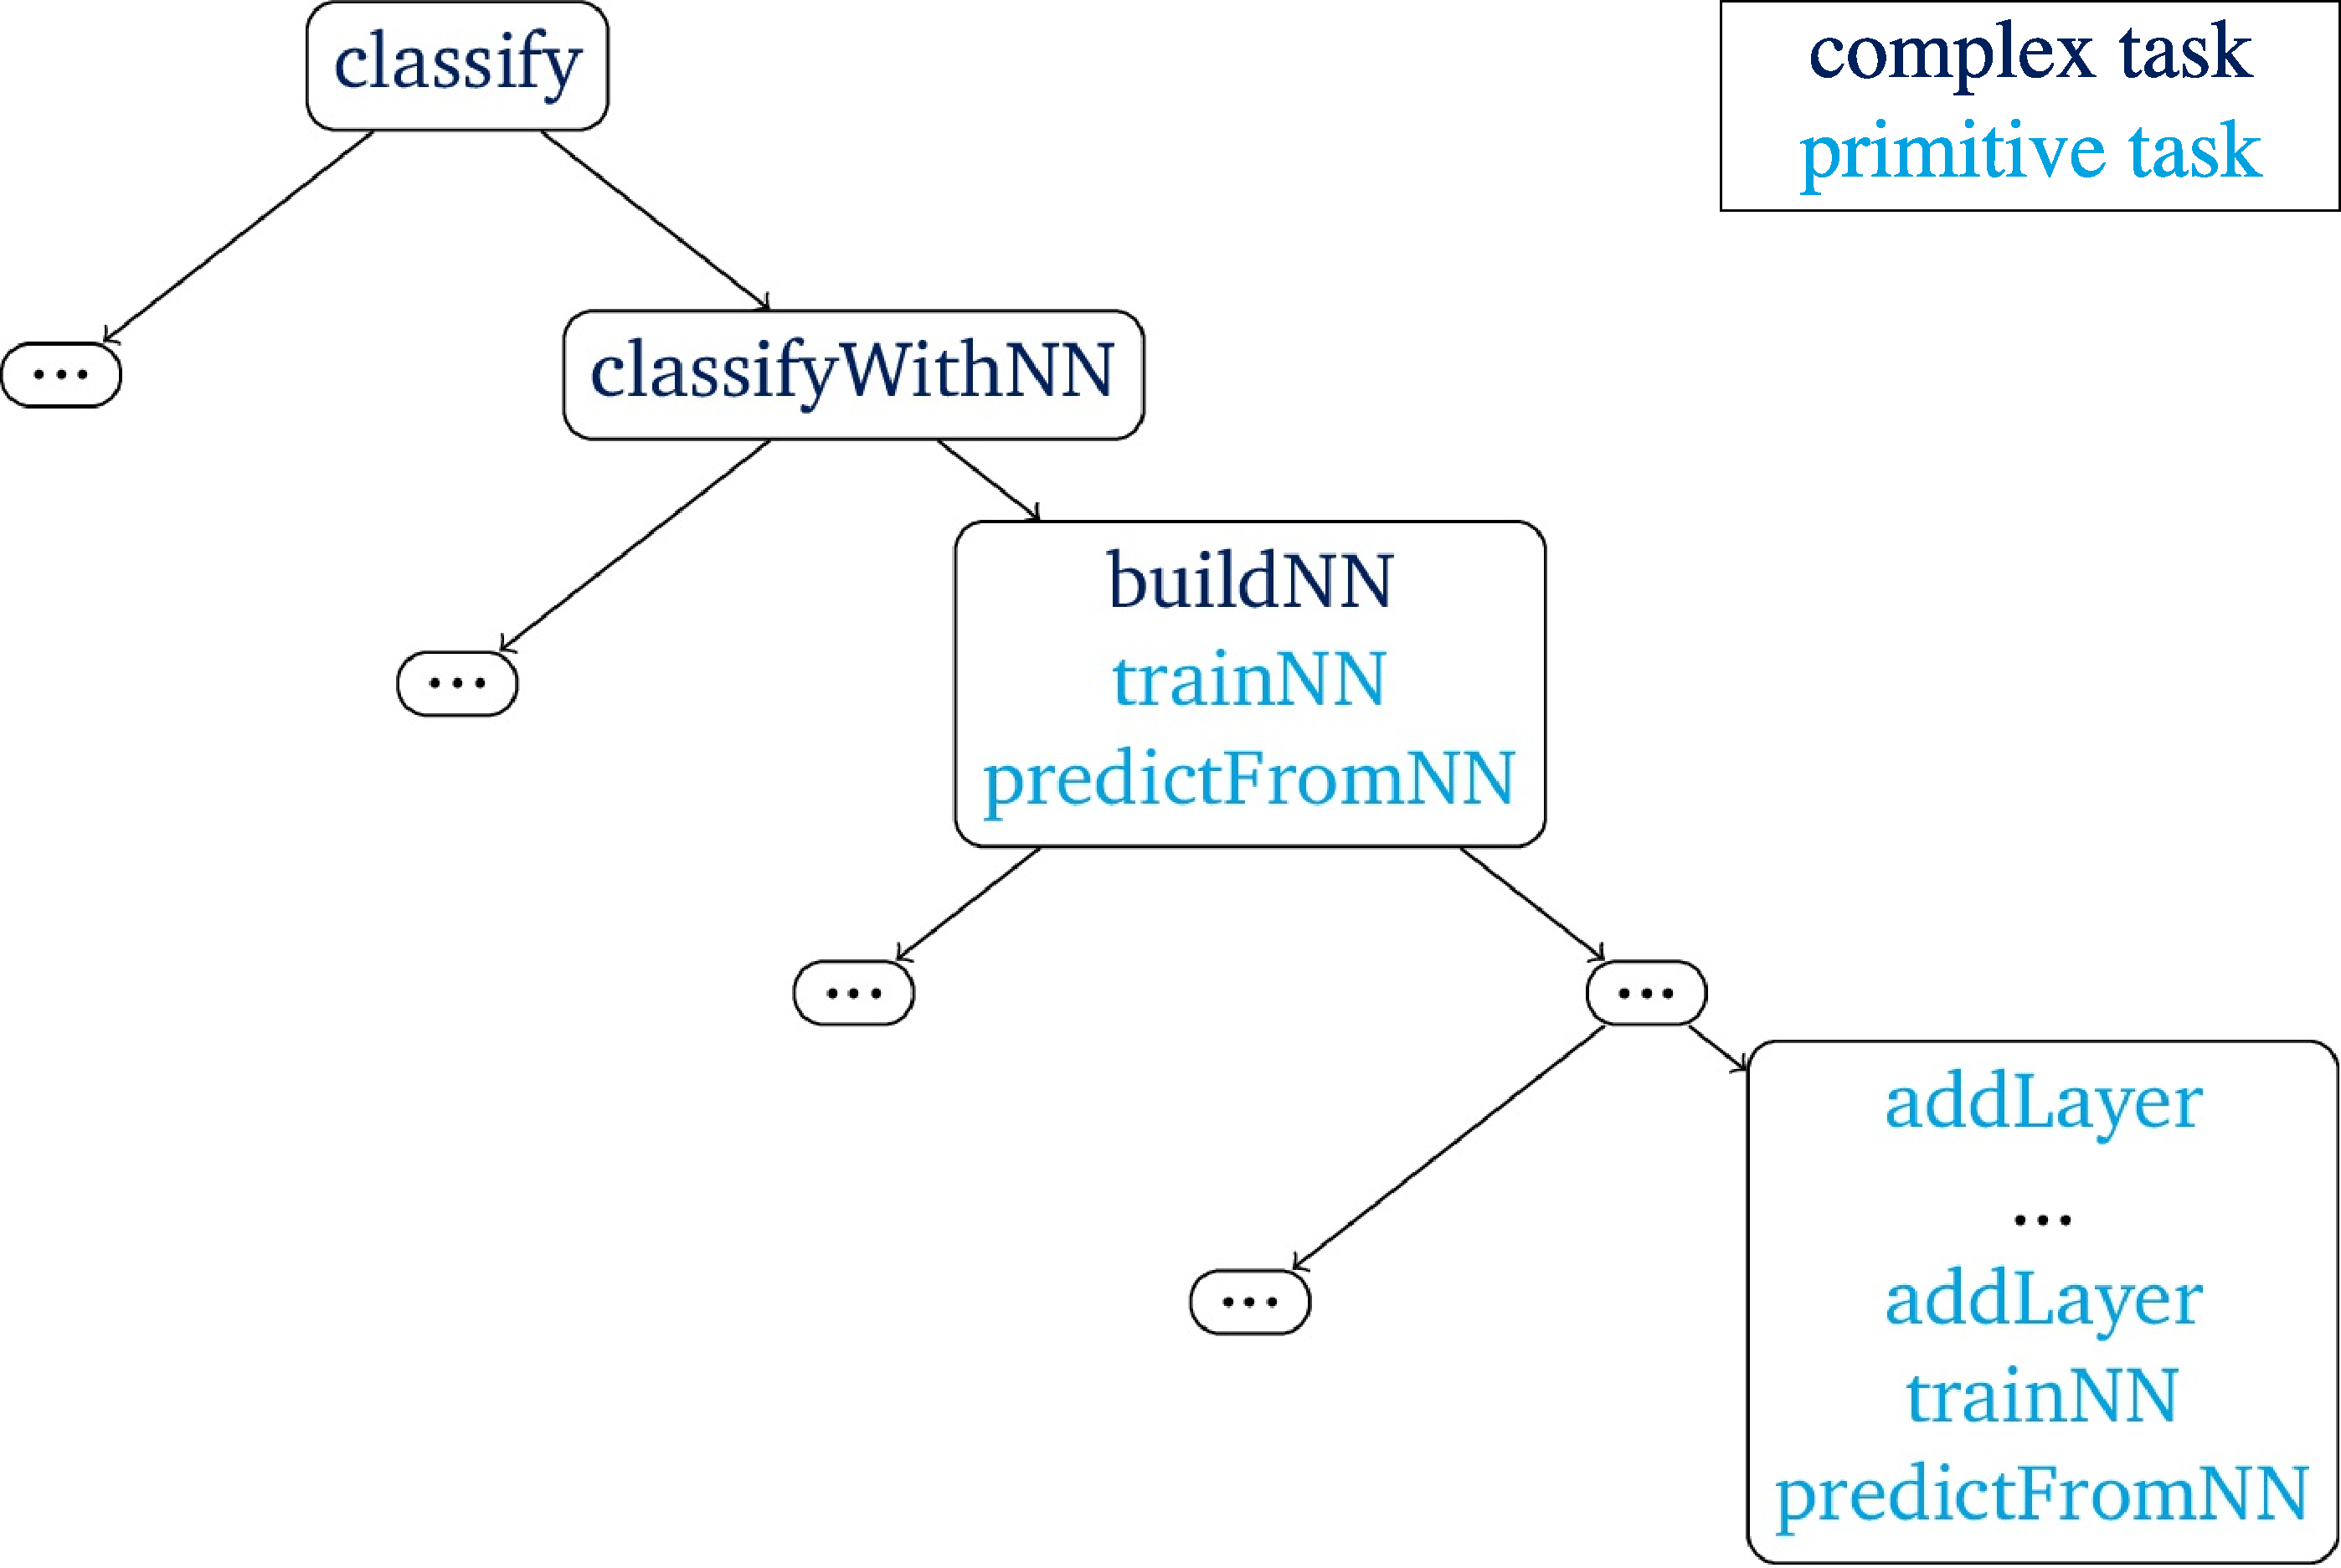
\includegraphics[width=.8\textwidth]{gfx/MLPlan.pdf}
\caption{An example for how the complex task 'classify' might be broken down by ML-Plan, adapted from \cite{wever2017automatic}. Nodes containing '...' represent an undefined number of subtrees.}
\label{fig:mltree}
\end{figure}

% Recipe framework
Similar to ML-PLAN, the RECIPE framework constructs whole classification pipelines for new problems \cite{DBLP:conf/eurogp/SaPOP17}. However, this is done by means of grammar-based genetic programming: the tasks that the pipeline is composed of are represented by a grammar, which 'is used to generate the initial population, as well as to constrain the crossover and mutation operations, which always need to be valid according to the grammar' \cite{DBLP:conf/eurogp/SaPOP17}. This means that generated individuals representing complete pipelines can never be invalid. So for a new data set combined with a grammar that represents the valid pipelines, the tool first initializes the first generation according to the grammar. The fitness of individuals is then evaluated by mapping them to their respective implementations in the scikit-learn framework, and a new generation is created that takes this newly gained information into account. Evaluation by the authors indicates that the RECIPE framework is able to compete with AUTO-SKLEARN and a different evolutionary approach, although it does not incorporate meta-knowledge in the search.